\documentclass[10pt,letterpaper]{article}

\providecommand{\main}{.}
\usepackage{cogsci}
\usepackage{pslatex}
\usepackage{graphicx}
\usepackage{multicol}
\usepackage{blindtext}
\usepackage{tablefootnote}
\usepackage{hyperref}
\usepackage{tipa}
\usepackage{booktabs}
\usepackage[table,usenames,dvipsnames]{xcolor}
\usepackage[style=apa]{biblatex}
\DeclareNameAlias{sortname}{family-given}
\addbibresource{qp1.bib}
\usepackage{gb4e}

\graphicspath{{\main/figures/}{figures}}

\title{`Sally the Congressperson': The Role of Individual Ideology on the Processing and Production of English Gender-Neutral Role Nouns}

\author{{\large \bf Brandon Papineau (branpap@stanford.edu)} \\\\
{\large \bf Robert J. Podesva (podesva@stanford.edu)} \\\\
{\large \bf Judith Degen (jdegen@stanford.edu)} \\
Department of Linguistics, Margaret Jacks Hall, Bldg. 460\\
Stanford, CA, 94305 USA}

\begin{document}
	
	\maketitle
	
	\begin{abstract} 
		Language and gender are inextricably linked; we make reference to the real-world gender identities of the people around us every day. Moreover, psycholinguistic investigation has demonstrated that we make assumptions about individuals' gender based on the language used to describe them, and that the biases underpinning these assumptions in turn influence the ways in which we describe and refer to others. What has been left underinvestigated is the role that individual, rather than societally-held, ideologies about gender play in this aspect of the linguistic system. In two web-based studies, we investigate the processing and production of gender-neutral role nouns such as \textit{congressperson} as a function of individual gender ideology and political alignment. Our results indicate an asymmetry between the processing and production of gender-neutral role nouns: while individuals' gender ideologies do not modulate the processing of these terms, gender ideologies do interact with political party in production tasks, such that Democrat-identified participants with more progressive gender ideologies produce more gender-neutral role nouns. We appeal to the notion of \textit{indexicality}, arguing that Democrats draw on these forms as semiotic resources for constructing progressive personae in interaction, while Republicans and political non-partisans do not.\\
		\linebreak
		\textbf{Keywords:} 
		language and gender; language processing; language production; language and politics; morphology
	\end{abstract}
	
	
	\section{Introduction}
	English contains a subset of lexical entries which identify the semantic or real-world gender identity of the individuals they pick out, consisting primarily of pronouns, kinship terms, and a limited set of other role nouns. While generally common in discourse, these terms are often ideologically, socially, and politically charged or contested. Consider the famous and contemporary case of English pronouns. While psycholinguistic investigations have indicated that there is a processing advantage found in singular \textit{they} when it is paired with gender-underspecified referents \parencite{foertsch1997search,doherty2017gender,ackerman}, its usage continues to be debated on the battlefields of style guides, op-eds, and popular discourse, especially as it relates to its use as a pronoun used by non-binary or gender non-conforming individuals.  \par 
	More conventionally-gendered pronouns have also been the subject of psycholinguistic analysis as they relate to real-world referent gender. \textcite{von2020implicit} found that, in the context of the United States 2016 presidential election, participant beliefs about whether or not Hillary Clinton would win the presidency had no effect on the production of \textit{she} as a coreferent pronoun with \textit{the future president}, and that \textit{she} induced a processing penalty when read in a context in which it was coreferent with \textit{the future president}. In fact, it was coreferential \textit{they} which increased in produced frequency as belief in Clinton's victory increased. However, in the context of the 2017 British General Election, \textit{she} was produced more frequently than \textit{he} when coreferential with \textit{the future Prime Minister}, when the incumbent Prime Minister was female (Theresa May). On the other hand, there was no such processing bonus for \textit{she} over \textit{he} until after the results of the election, indicating lingering sexist beliefs in the realm of language processing. These findings are reminiscent of previous work examining the relationship between societal expectations and reading times on gender-anomalous coreferents. For instance, coreferential pronouns are harder to process when they do not align with the stereotypical gender of the role noun in question, such as \textit{he} for \textit{nurse} or \textit{she} for \textit{electrician} \parencite{foertsch1997search,duffy2004violating}. These findings, taken together, suggest that our biases about who performs a particular social role inform the ways we produce and process the pronouns which refer to them.\par 	
	Beyond the realm of pronominal reference, \textcite{pozniak2021failures} found that respondents who believed that female candidates would win in the 2020 Parisian and Marseille municipal elections were more likely to produce feminine-marked titles (as well as pronouns) to refer to the future politicians, but that masculine-marked forms were still dominant in both locales. Corpus data similarly indicates that referent gender indication is more prevalent when the gender of the referent runs counter to stereotypical assumptions. For example, the Corpus of Contemporary American English \parencite{coca} contains 165 tokens of \textit{male nurse}, compared to 53 of \textit{female nurse}. These biases are in turn learned by large language models trained on natural language corpora, raising concerns about the perpetuation of societal biases in the realm of automation and language \parencite{caliskan2017semantics,bender2021dangers,sutton2018biased}. Such findings further underscore the role of societally-held beliefs about the genders of particular social roles play in the language we use to describe those who fill these roles.\par 
	While the aforementioned studies have investigated the role of group and societal-level biases in the processing and production of gendered language, this high-level focus leaves room for a more granular investigation of the role of \textit{individual} ideologies on this facet of the linguistic system. We can couch this question in the notion of surprisal, which measures processing difficulty as proportional to the relative surprisal (1) of a particular word occurring given previous input (\textit{w}\textsubscript{1},...,\textit{w}\textsubscript{\textit{i}-1}) and any extralinguistic or extrasentential content (\textit{C}) \parencite{levy2008expectation}.
	
	\begin{exe}
		\item processing difficulty $\propto$ log\textit{P}(\textit{w}\textsubscript{\textit{i}}$|$\textit{w}\textsubscript{1},...,\textit{w}\textsubscript{\textit{i}-1},\textit{C})
	\end{exe}
	
	In the aforementioned examples, we can explain processing difficulties incurred by co-referring pronouns that do not concord with stereotypical associations of particular occupations by positing that these pronouns are relatively more surprising than would be a stereotype-concordant pronoun, as a result of prior beliefs about gender roles. However, it is reasonable to assume that not every individual will interpret these co-referential terms as being equally surprising. For example, we might expect that an individual with a particularly open-minded attitude towards gender roles will be socially progressive and consume media that reflects these values; as a result, they may be exposed to more gender-neutral language, and in turn less surprised by its use in context. Alternatively, the ideologies themselves might be at play in the calculation of difficulty, in the form of extrasentential context. \par 
	While it may be difficult to tease apart exactly where ideology is implemented in processing calculations, we set out to investigate the \textit{extent} to which such individually-held ideologies might influence the processing and production of gender-neutral language, and how they might manifest. We conducted two web-based experiments centered around the domain of `role nouns', which describe individuals' social and professional positions in the world \parencite{misersky2014norms}. These include both compound forms (n=14) which make a ternary distinction between male, female, and gender-neutral forms, as well as affixed forms which make only a binary distinction (n=6). Examples of these forms are provided in (1) and (2), respectively.
	
	\begin{exe}
		\ex \textbf{Compound ternary distinctions}
		\begin{xlist}
			\ex \textit{congressman, congresswoman, congressperson}; \textit{policeman, policewoman, police officer}
		\end{xlist}
		\ex \textbf{Affixed binary distinctions}
		\begin{xlist}
			\ex \textit{actor, actress}; \textit{villain, villainess}
		\end{xlist}
	\end{exe}
	
	We report on the experimental design and results of two studies: Experiment 1 examines whether the processing of gender-neutral nouns is modulated by individuals' gender ideology, while Experiment 2 examines whether this same ideology affects the production of these terms. We conclude with a discussion of how these findings contribute to our understanding of the gender-language relationship \footnote{It is important to note that many of the assumptions in our designs, such as the decision to use `male' and `female' names, implicitly endorse or perpetuate the notion of gender as a binary. We would like to highlight that these decisions in no way reflect the beliefs or values of the authors.}.\par 
	
	
	\section{Experiment One: Self-Paced Reading}
	In an experiment similar to that of the processing experiment in \textcite{von2020implicit}, our first investigation concerned the role that individuals' ideologies about gender play in their processing of gender-neutral role nouns.
	
	
	\subsection{Methods}
	\subsubsection{Participants}
	298 participants were recruited through the online recruitment platform \textcite{prolific}\footnote{200 participants were initially recruited, and an additional 98 Republican participants were subsequently recruited after the original sample revealed a heavy skew towards Democrat-identifying participants.}, excluding any participants who failed to correctly respond to at least 85\% of attention check questions (n=19). All participants additionally self-identified as L1 English speakers and as having been born and in and currently residing in the United States. None of the participants had participated in the pilot study or in any other study related to the present project. The demographic breakdown of the participants whose data was included in Experiment One is provided in \hyperref[exp1-sample-table]{Table 1}.\par 
	
		\begin{table}[!ht]
		\begin{center} 
			\caption{Experiment One Participant Demographics} 
			\label{exp1-sample-table} 
			\vskip 0.12in
			\begin{tabular}{llll} 
				\hline
				&  Democrat & Republican & Non-Partisan\tablefootnote{In both studies, `Non-Partisan' participants were recruited as either Democrats or Republicans, but reported a centrist identity in the post-experimental questionnaire.} \\
				\hline
				Female &  64 & 41 & 34 \\
				Male & 46 & 59 & 25 \\
				Other & 3 & 0 & 0 \\
				Decline to state & 0 & 3 & 1 \\
				\hline
			\end{tabular} 
		\end{center} 
	\end{table}

	\subsubsection{Stimuli \& Procedure} In a web-based implementation of a self-paced reading task, participants saw a series of 20 sentence sets of the form ``[NAME] is a(n) [TITLE] from [STATE]. S/he likes [ACTIVITY]", where ``[TITLE]" stands in for the critical item of gendered role noun. The states and activities were randomized at the stimuli creation stage so that they remained constant for all participants. On the other hand, names varied such that each participant saw 10 vignettes with male-coded names and 10 with female-coded names. Role nouns were then distributed so that 5 of the female names co-occurred with female-marked forms and the other 5 with neutral forms; the same was true for the male names, but with male-marked forms\footnote{We intentionally avoided gender-incongruent forms such as `David is a congresswoman', for fear that doing so would bring too much attention to the research question regarding gender.}. The resulting combinations are presented in (3) through (6); participants saw each of these combinations five times, followed by activity preferences, for a total of twenty trials. Each name and title occurred only once, so that no participant saw both `congressman' and `congresswoman' or `congressperson', for example'.
	
	\begin{exe}
		\ex \textbf{\textit{Female congruent }}
		\begin{xlist}
			\ex Sally is a congresswoman from Kansas.
		\end{xlist}
			\ex \textbf{\textit{Female neutral}}
		\begin{xlist}
			\ex Sally is a congressperson from Kansas. 
			\end{xlist}
				\ex \textbf{\textit{Male congruent }}
		\begin{xlist}
			\ex David is a congressman from Kansas. 
		\end{xlist}
		\ex \textbf{\textit{Male neutral}}
		\begin{xlist}
			\ex David is a congressperson from Kansas. 
		\end{xlist}
	\end{exe}
	
	  In order to attain sufficiently-gendered names, the twenty most popular male and female names were selected from the lists of most popular names for boys and girls in 1998 according to the United States Social Security \textcite{socialsecurity}. Names which appeared within the top 100 entries on both lists (e.g. Taylor, Ryan) were excluded. \par 
	  Participants proceeded through these sentences one word at a time by pressing the spacebar. This resulted in the previous word disappearing and the subsequent one being revealed on the screen; measurements of reading time were taken for each word in the sentence as a proxy for processing difficulty or effort, as has been standardized in the field \parencite{forster2009maze}. At the end of each vignette, participants were asked about properties of the character described, providing a `yes' or `no' answer to questions about their home state (\textit{Is Sally from Kansas?}) or about their preferred activities (\textit{Does David enjoy skiing?}); these questions served both to distract from the principal question under investigation, and as attention checks, since each of these questions had a vignette-internally correct answer. Participants were provided with an example that did not mark gender before proceeding to the main set of 20 vignettes. 
	  
	\subsubsection{Post-Experimental Survey} 
	Upon completing the reading task, participants proceeded to the post-experimental survey. \par 
	In order to assess the participants' ideologies towards gender, we employ the Social Roles Questionnaire developed by \textcite{baber2006social}. This survey consists of 13 questions which are designed to elicit both implicit and explicit ideologies about gender, including the notions of gender as an immutable fact vs gender as a social construct (what Baber and Tucker term `gender transcendence'), as well as about the societal roles performed by the (binary) genders (`gender linking').\par 
	Each of the 13 questionnaire items was presented alongside a sliding scale from `strongly disagree' to `strongly agree', which corresponded to numerical values of 0 and 100, respectively. The questions related to `gender linking' were inversely coded and then converted to the same scaling as the `gender transcendence' subscale. Participants were then assigned a gender ideology score from 0 to 100 by taking the mean of their individual responses; the closer to 0 a participant is, the more open-minded their approach to gender, and the closer to 100, the more conservative or traditional their view of gender. These opposite poles of the spectrum were termed `gender progressive' and `gender conservative', respectively.\par 
	Finally, participants filled out an optional post-experimental demographic survey, including questions about their own gender, political affiliations, and age. Participants who declined to indicate their age or political orientation were excluded from analysis.
	
	\subsubsection{Unigram Surprisal}
	In order to account for effects of word frequency and surprisal, frequency values for each of the twenty critical items' neutral forms were taken from the `Spoken' (news media) section of COCA \parencite{coca}. These were then converted into unigram surprisal values by taking the negative log of their relative probabilities in the corpus. The decision to use unigram, contextless surprisal values was due to the difficulty in using large language models to obtain surprisal values for very infrequent terms, such as \textit{foreperson}. 
	
	\subsection{Results}
	
	\subsubsection{Exclusions}
	In addition to the aforementioned participant exclusions, 238 trials were excluded for being more than 2.5 standard deviations away from that lexical item's mean reading time, resulting in a final count of 5,342 observations for analysis (4.2\% exclusion rate).
	
	\subsubsection{Model Structure} 
	We fit a linear mixed effect model which predicted length-residualized reading time from fixed effects of political party (ternary, reference level: ``Democrat"), referent gender (binary, reference level: ``female"), participant age, gender ideology, and unigram surprisal. Random intercepts were included for participant and lexeme. Interactions were included between: ideology and age; surprisal and party; age and surprisal; age and party; ideology and party, and the three-way interaction between age, surprisal, and party. These interactions were included as a result of initial investigations which revealed a significant modulation of frequency effects by age (Figure 3).
	
	\subsubsection{Gender Ideology} In examining the role of gender ideology in the processing of gender-neutral terms, we find no effect of gender ideology for Democrats ($\beta$ = -0.00, \textit{SE} = 0.00, \textit{t} = -0.11, \textit{p} $>$ 0.5), or in the higher-level interactions for Republicans ($\beta$ = -0.00, \textit{SE} = 0.00, \textit{t} = -1.51, \textit{p} $>$ 0.1) or Non-Partisans ($\beta$ = -0.00, \textit{SE} = 0.00, \textit{t} = -1.34, \textit{p} $>$ 0.1), suggesting that prior beliefs about gender and its binary social roles does not modulate the processing of gender-neutral language.
	
	\begin{figure}[h]
		\centering
		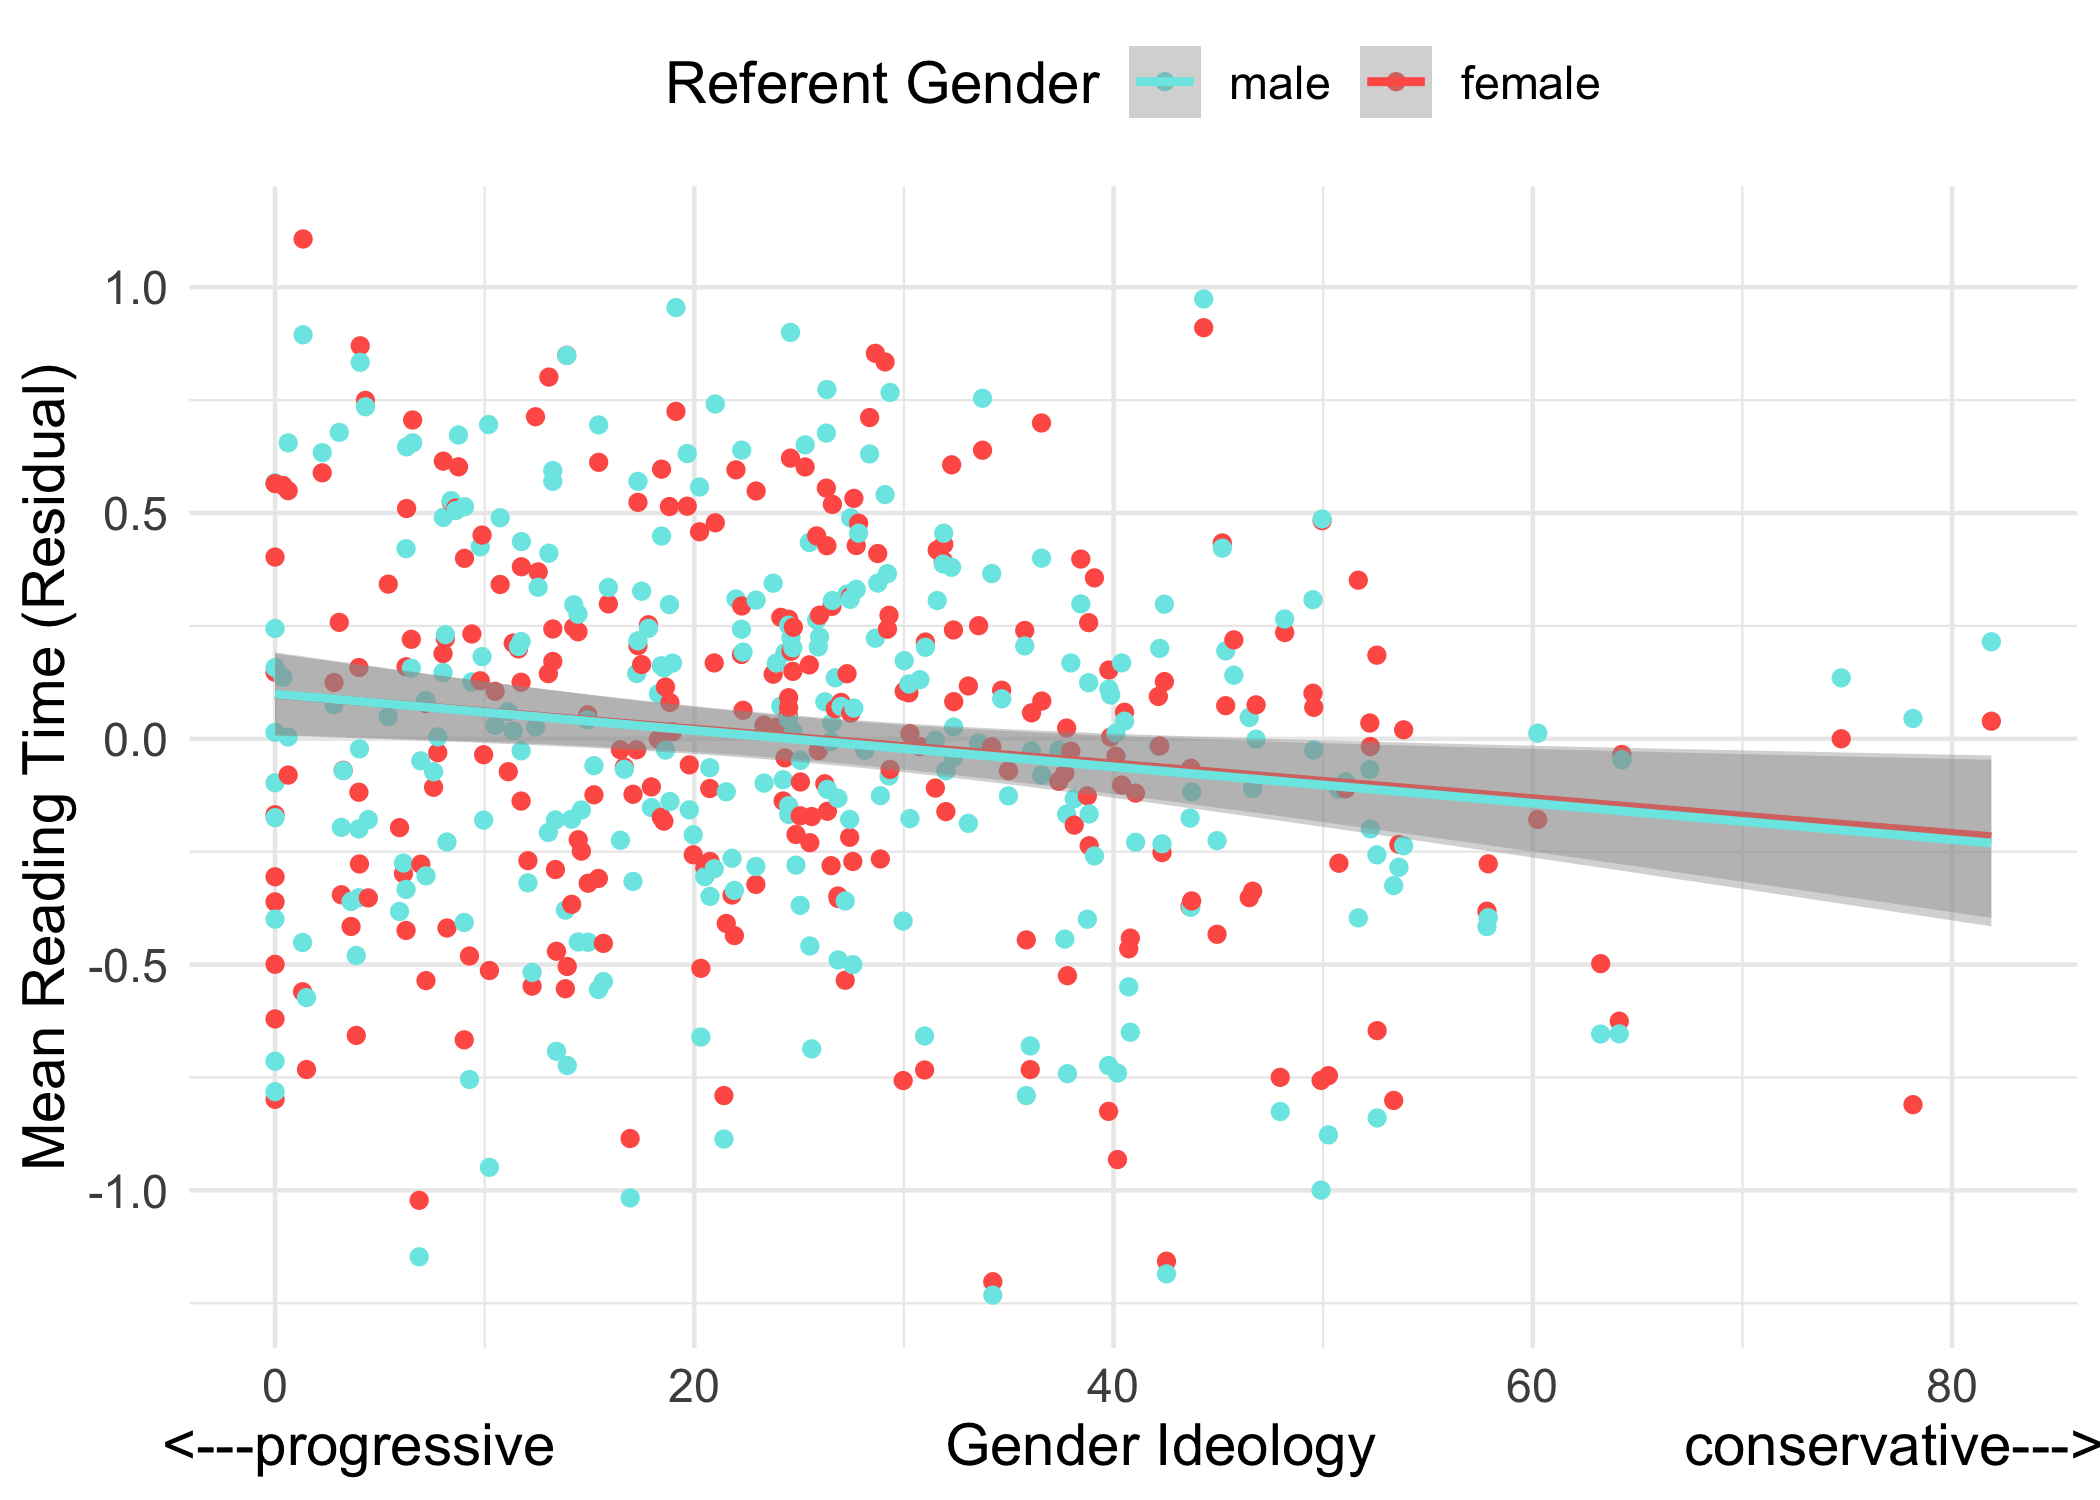
\includegraphics[scale=0.115]{sprt-neutral-ideo.png}
		\caption{Residualised reading time on neutral forms (e.g. \textit{congressperson}) as a function of gender ideology}
	\end{figure}
	
	\subsubsection{Political Affiliation}
	At the party-level, we find that Democrats are significantly faster than their Non-Partisan counterparts in their reading of gender-neutral terms ($\beta$ = 0.04, \textit{SE} = 0.02, \textit{t} = 2.354, \textit{p} = 0.02), but this difference is not found between Democrats and Republicans ($\beta$ = 0.00, \textit{SE} = 0.02, \textit{t} = 0.83, \textit{p} $>$ 0.1). However, we observe the same difference between Democrats and Non-Partisans in the sentences prefixes leading up to the critical items, as shown in the first three points of Figure 1. As a result, we interpret this a spurious result unrelated to ideology and its affect on processing times.
	
	\begin{figure}[h]
		\centering
		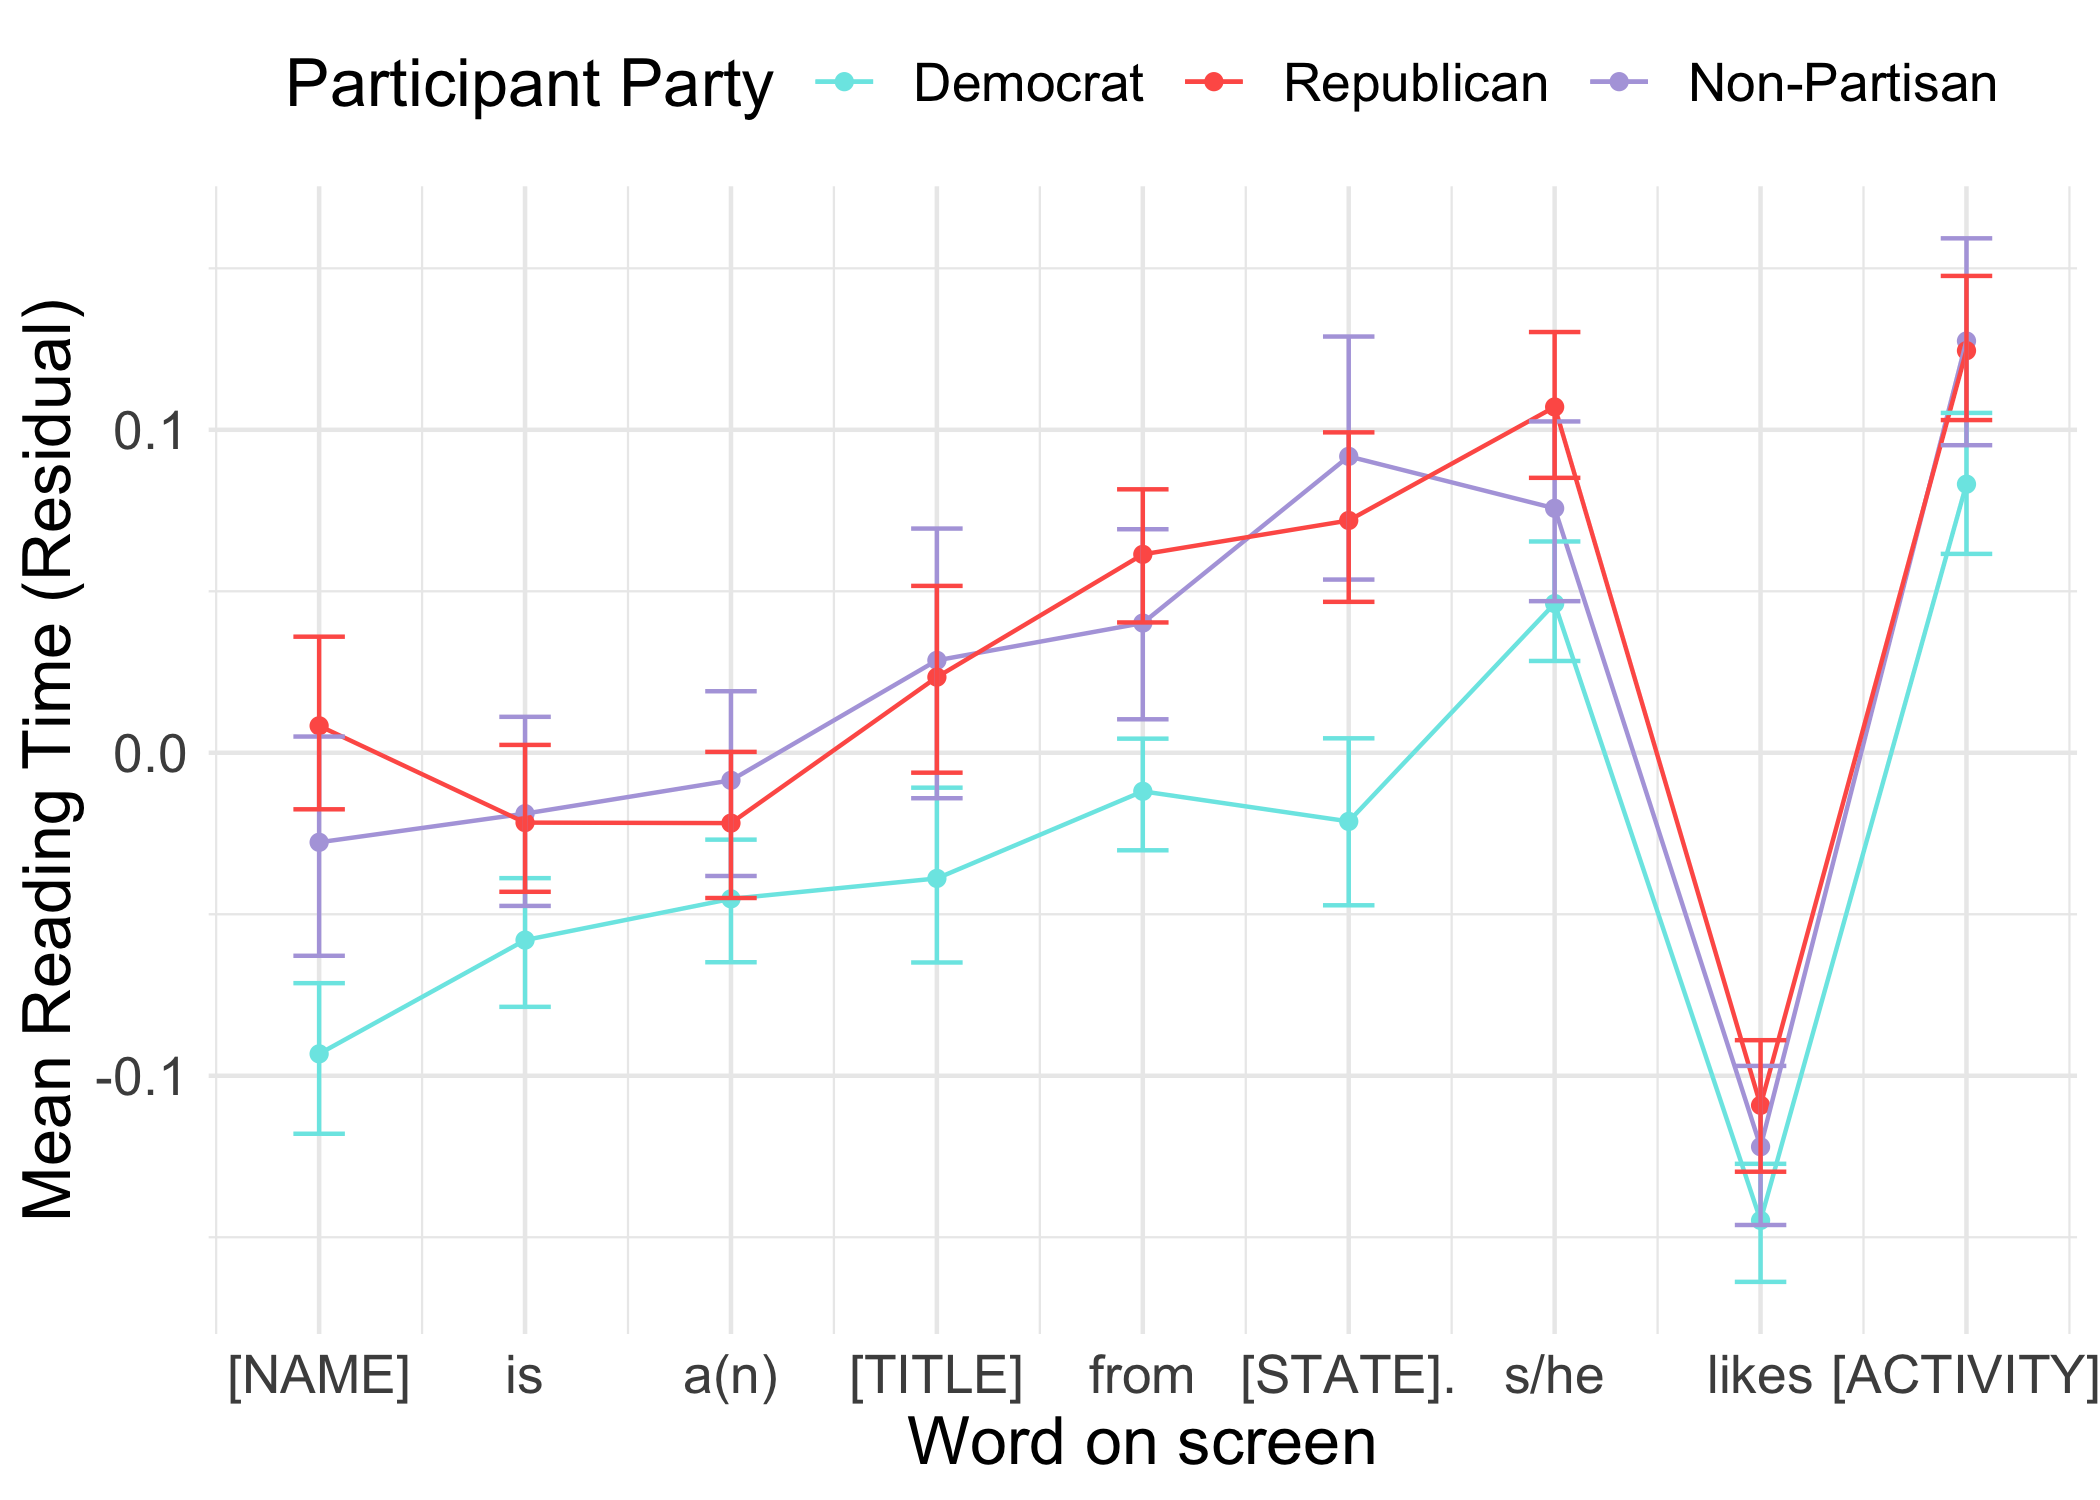
\includegraphics[scale=0.115]{sprt-neutral-all-regions-poli-party.png}
		\caption{Residualised reading time by sentence location. ``[TITLE]" indicates the location of the critical items.}
	\end{figure}


	\subsubsection{Unigram Surprisal}
	Finally, we find only a marginal effect of word surprisal ($\beta$ = -0.02, \textit{SE} = 0.01, \textit{t} = -1.825, \textit{p} = 0.07). Despite this, we do find that there is a significant three-way interaction in the Democratic party ($\beta$ = 0.00, \textit{SE} = 0.00, \textit{t} = 2.378, \textit{p} = 0.02) and that Republicans do not significantly differ from them ($\beta$ = -0.00, \textit{SE} = 0.0, \textit{t} = -0.78, \textit{p} = 0.43), such that older participants show a greater degree of sensitivity to word surprisal in the expected direction; more surprising words are processed more slowly. This effect is weaker in younger Republicans, however, and entirely absent in younger Democrats (Figure 3). This may indicate that the frequency values obtained from COCA are not representative of the linguistic input experienced by younger Americans.
	
	\begin{figure}[h!]
		\centering
		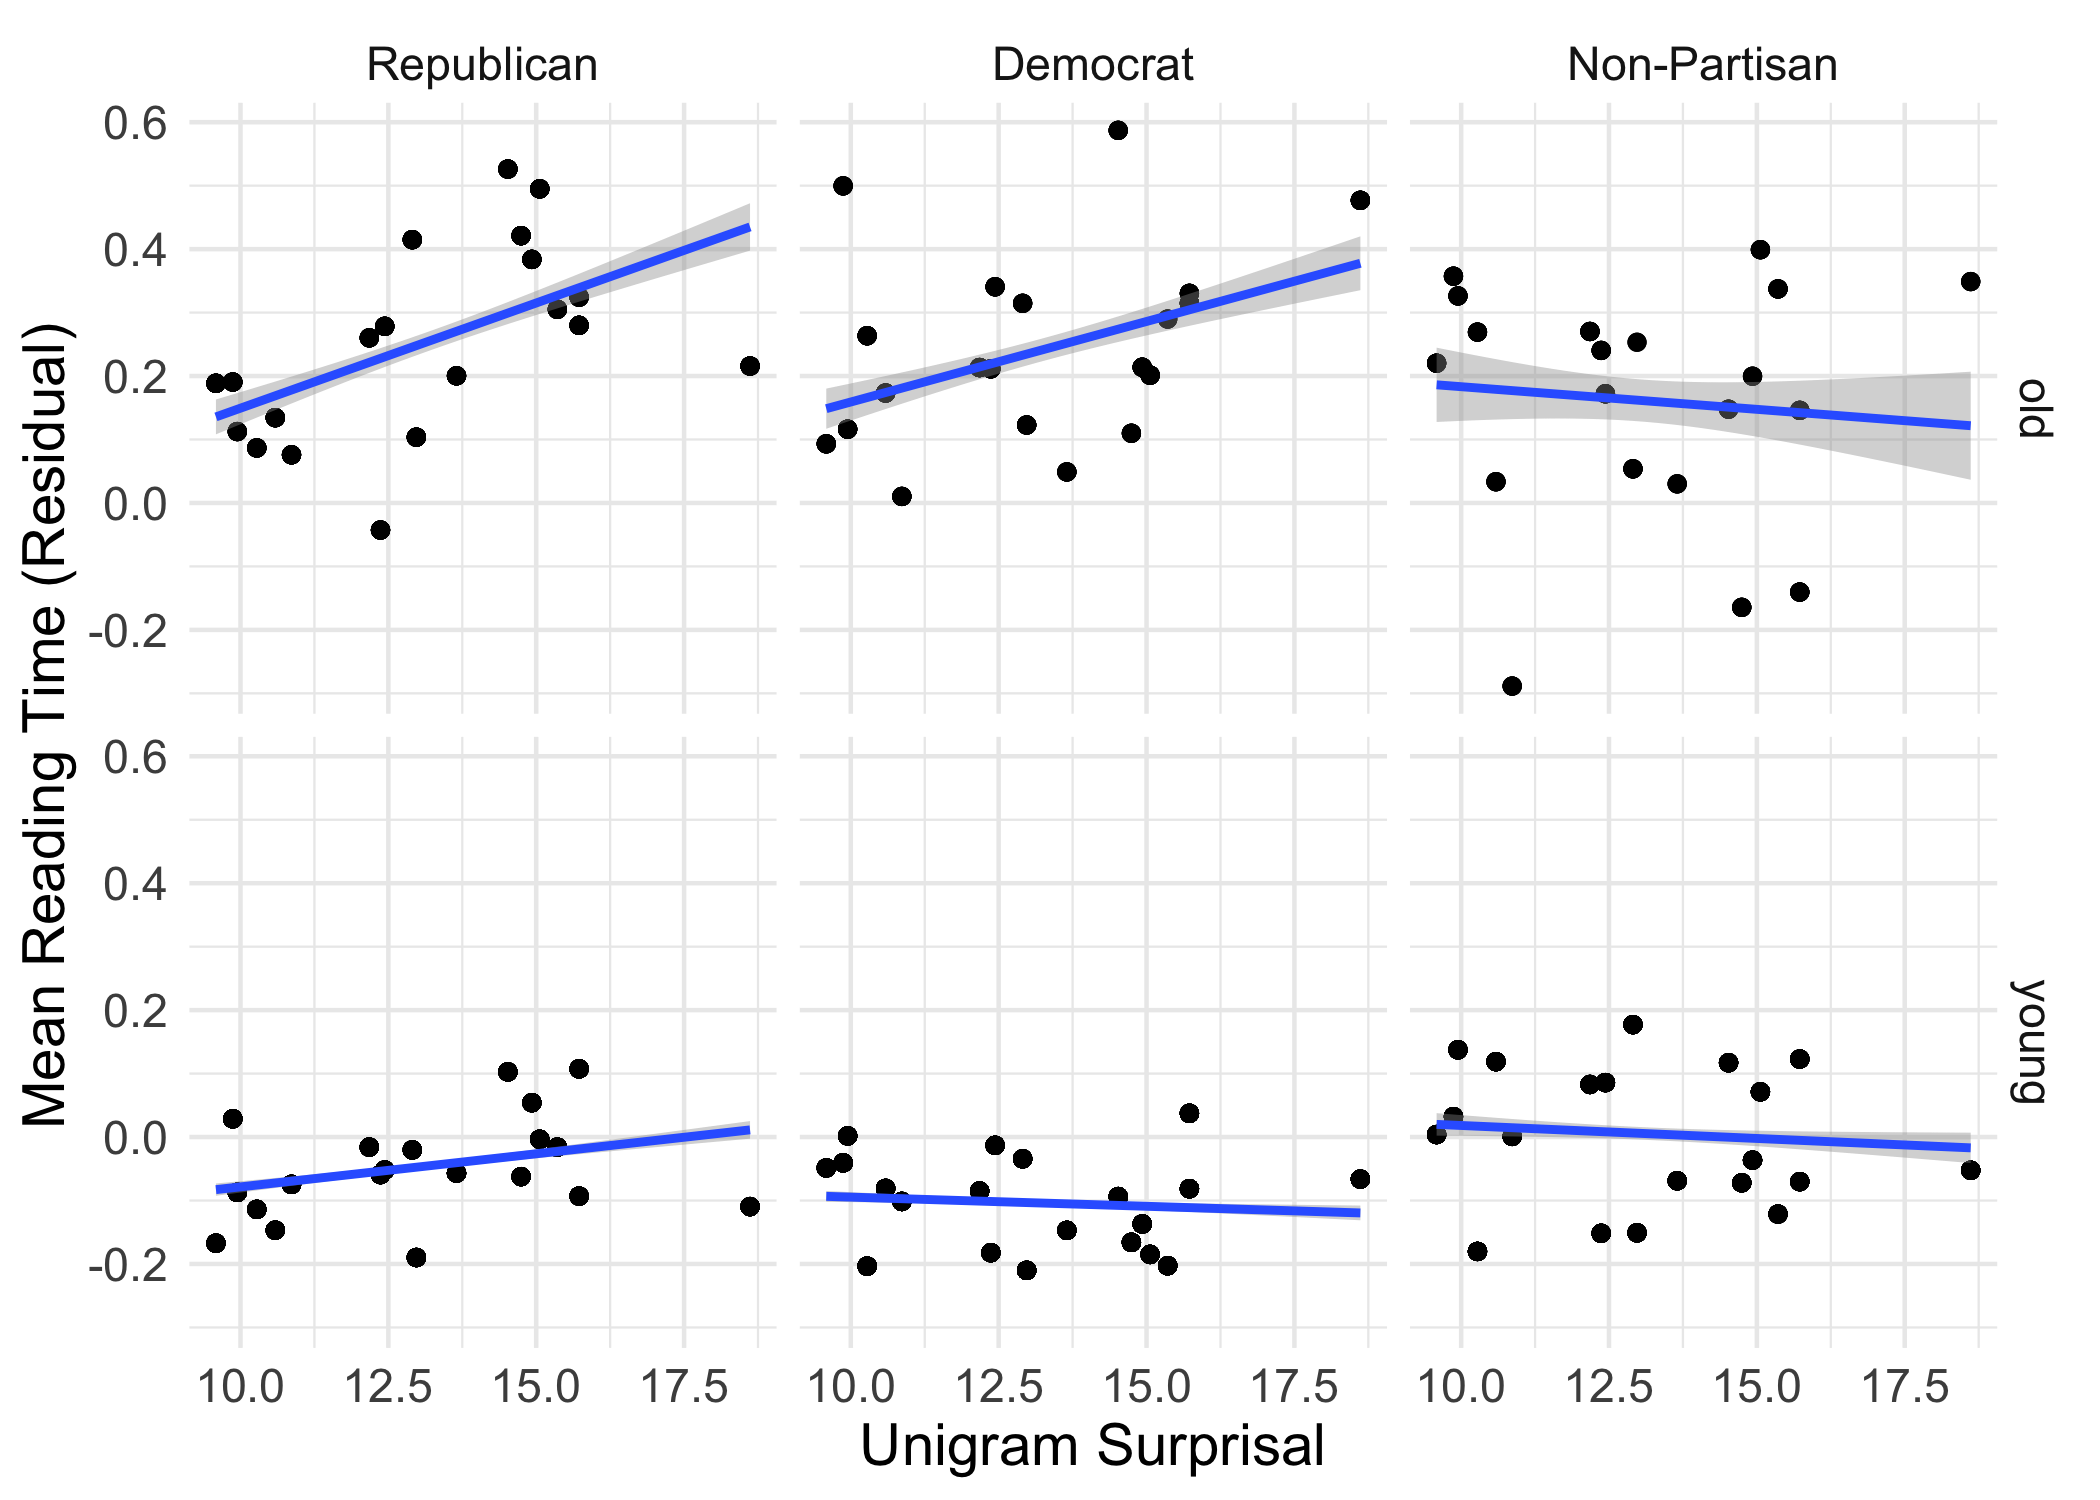
\includegraphics[scale=0.115]{proc-freq-party.png}
		\caption{Residualised reading time on critical items by log word frequency. Each point indicates a lexeme.}
	\end{figure}
	
	\section{Experiment Two: Forced-Choice Production}
	Having investigated the potential link between gender ideology and the processing of neutral role nouns, we turn to the issue of ideology and the production of such terms. In a forced-choice task, participants selected the form of the lexeme they felt best completed the vignettes from Experiment One.
	
	\subsection{Methods}
	\subsubsection{Participants} 301 participants were recruited using Prolific, with the same criteria as Experiment 1\footnote{100 Democrats and 100 Republicans were recruited initially, in order to maintain a political balance. An additional 100 male-identifying participants were subsequently recruited due to a significant gender imbalance in the initial participant population (13.4\% male-identifying participants in the original population), as a result of an influx of female participants after Prolific went viral on social media app TikTok \parencite{charalambides2021}.}. Participants who failed to correctly respond to 80\% of attention checks were excluded (n=25). The final gender-political distribution is provided in \hyperref[exp2-sample-table]{Table 2}.\par

	\begin{table}[!ht]
		\begin{center} 
			\caption{Experiment Two Participant Demographics} 
			\label{exp2-sample-table} 
			\vskip 0.12in
			\begin{tabular}{llll} 
				\hline
				&  Democrat & Republican & Non-Partisan \\
				\hline
				Female &  82 & 62 & 25 \\
				Male & 42 & 46 & 10 \\
				Other & 4 & 0 & 0 \\
				Decline to state & 1 & 0 & 1 \\
				\hline
			\end{tabular} 
		\end{center} 
	\end{table}
	
	\subsubsection{Stimuli \& Procedure} All items in the experiment consisted of a complete sentence missing a single word, using the same stimuli sentence frames and critical items from Experiment One. Participants were then provided with either two or three words which could complete the sentence by filling in the blank, and were asked to select the word which best did that. There were a total of 80 trials, with 20 critical items and 60 filler items.\par 
	Filler items took one of two forms; semantic fillers and grammatical fillers. Semantic fillers had no prescriptively correct answer, and employed items from the same semantic field (7) or made use of common idioms or sayings (8). Some of these questions also dealt specifically with social and occupational titles and adopted the same syntactic frame as the critical items, in order to distract from the salience of gender in the critical items (9). 
	
	\begin{exe}
		\ex That's the cutest (horse/Lusitano/equine) I have ever seen!
		\ex The (customer/parent/child) is always right.
		\ex Revati is a (writer/journalist/author) from India.
	\end{exe}
	
	Grammatical fillers, on the other hand, had prescriptively correct answers, and employed grammatical processes such as demonstrative selection (10), verb agreement (11), or preposition selection (12), among others. These items served a secondary purpose as attention check questions.
	
	\begin{exe}
		\ex She is typing on (\textbf{the}/these/those) computer.
		\ex Katherine (\textbf{sang}/song/sing) that song beautifully. 
		\ex They are they eating their soup (between/\textbf{with}/at) a spoon.
	\end{exe}
	
	All response possibilities, regardless of type (filler or critical) were shuffled between participants to control for possible ordering effects of presented options. As such, the examples in (1)-(6) are not necessarily indicative of the orders in which options were presented to participants. Similarly, all 70 trials were randomized between participants, after which they moved to the post-experimental phase of the study. 
	
	\subsubsection{Post-Experiment Questionnaire}
	All participants completed the same post-experiment questionnaire as that of Experiment One. 
	
	\subsubsection{Log Odds} 
	Similar to the frequency values incorporated in the analysis of Experiment One, we calculated a rough probability value for each of the neutral terms given its co-occurrence with a particular name gender. Because participants were presented with both gendered and gender-neutral options, traditional frequency values are insufficient to capture the probability of a particular form being selected. As a result, log odds were calculated as the log proportion of neutral forms over the competing gendered form, given a particular gendered name, with words per million values taken from the `spoken' portion of the Corpus of Contemporary American English \parencite{coca}. For example, in the sentence `Sally is a congress[person/woman/man]', the log odds of `congressperson' are calculated as the words per million occurrences of `congressperson' divided by the same metric for `congresswoman'. This measure was then included in the final models used for analysis.
	
	
	\subsection{Results}
	
	\subsubsection{Exclusions} 
	An additional 241 responses were excluded from analysis for being incongruent with the names that appeared in the vignettes, such as `David is a congresswoman' or `Sally is a congressman'. These responses are, however, included in the visualizations presented in this section. This set of exclusions leaves us with a final set of 5179 analyzable observations.
	
	\subsubsection{Gender Ideology} We did not observe a main effect of gender ideology on the proportion of gender-neutral responses selected. Rather, only Democrats show an effect of this predictor, such that more gender progressive Democrats produced higher proportions of gender-neutral role nouns than their less progressive counterparts. Republicans and Non-Partisans show no such modulation by gender ideology. These observations are presented in Row 2 of Table 3. \par 
	We additionally find that Democrats have a higher base production rate of gender-neutral role nouns than their Non-Partisan or Republican counterparts. While Democrats selected the gender-neutral forms 59.6\% of the time, Republicans selected them only 45.1\% of the time. The political Non-Partisans performed in the middle, selecting the neutral forms 53\% of the time.
	
	\begin{figure}[h]
		\centering
		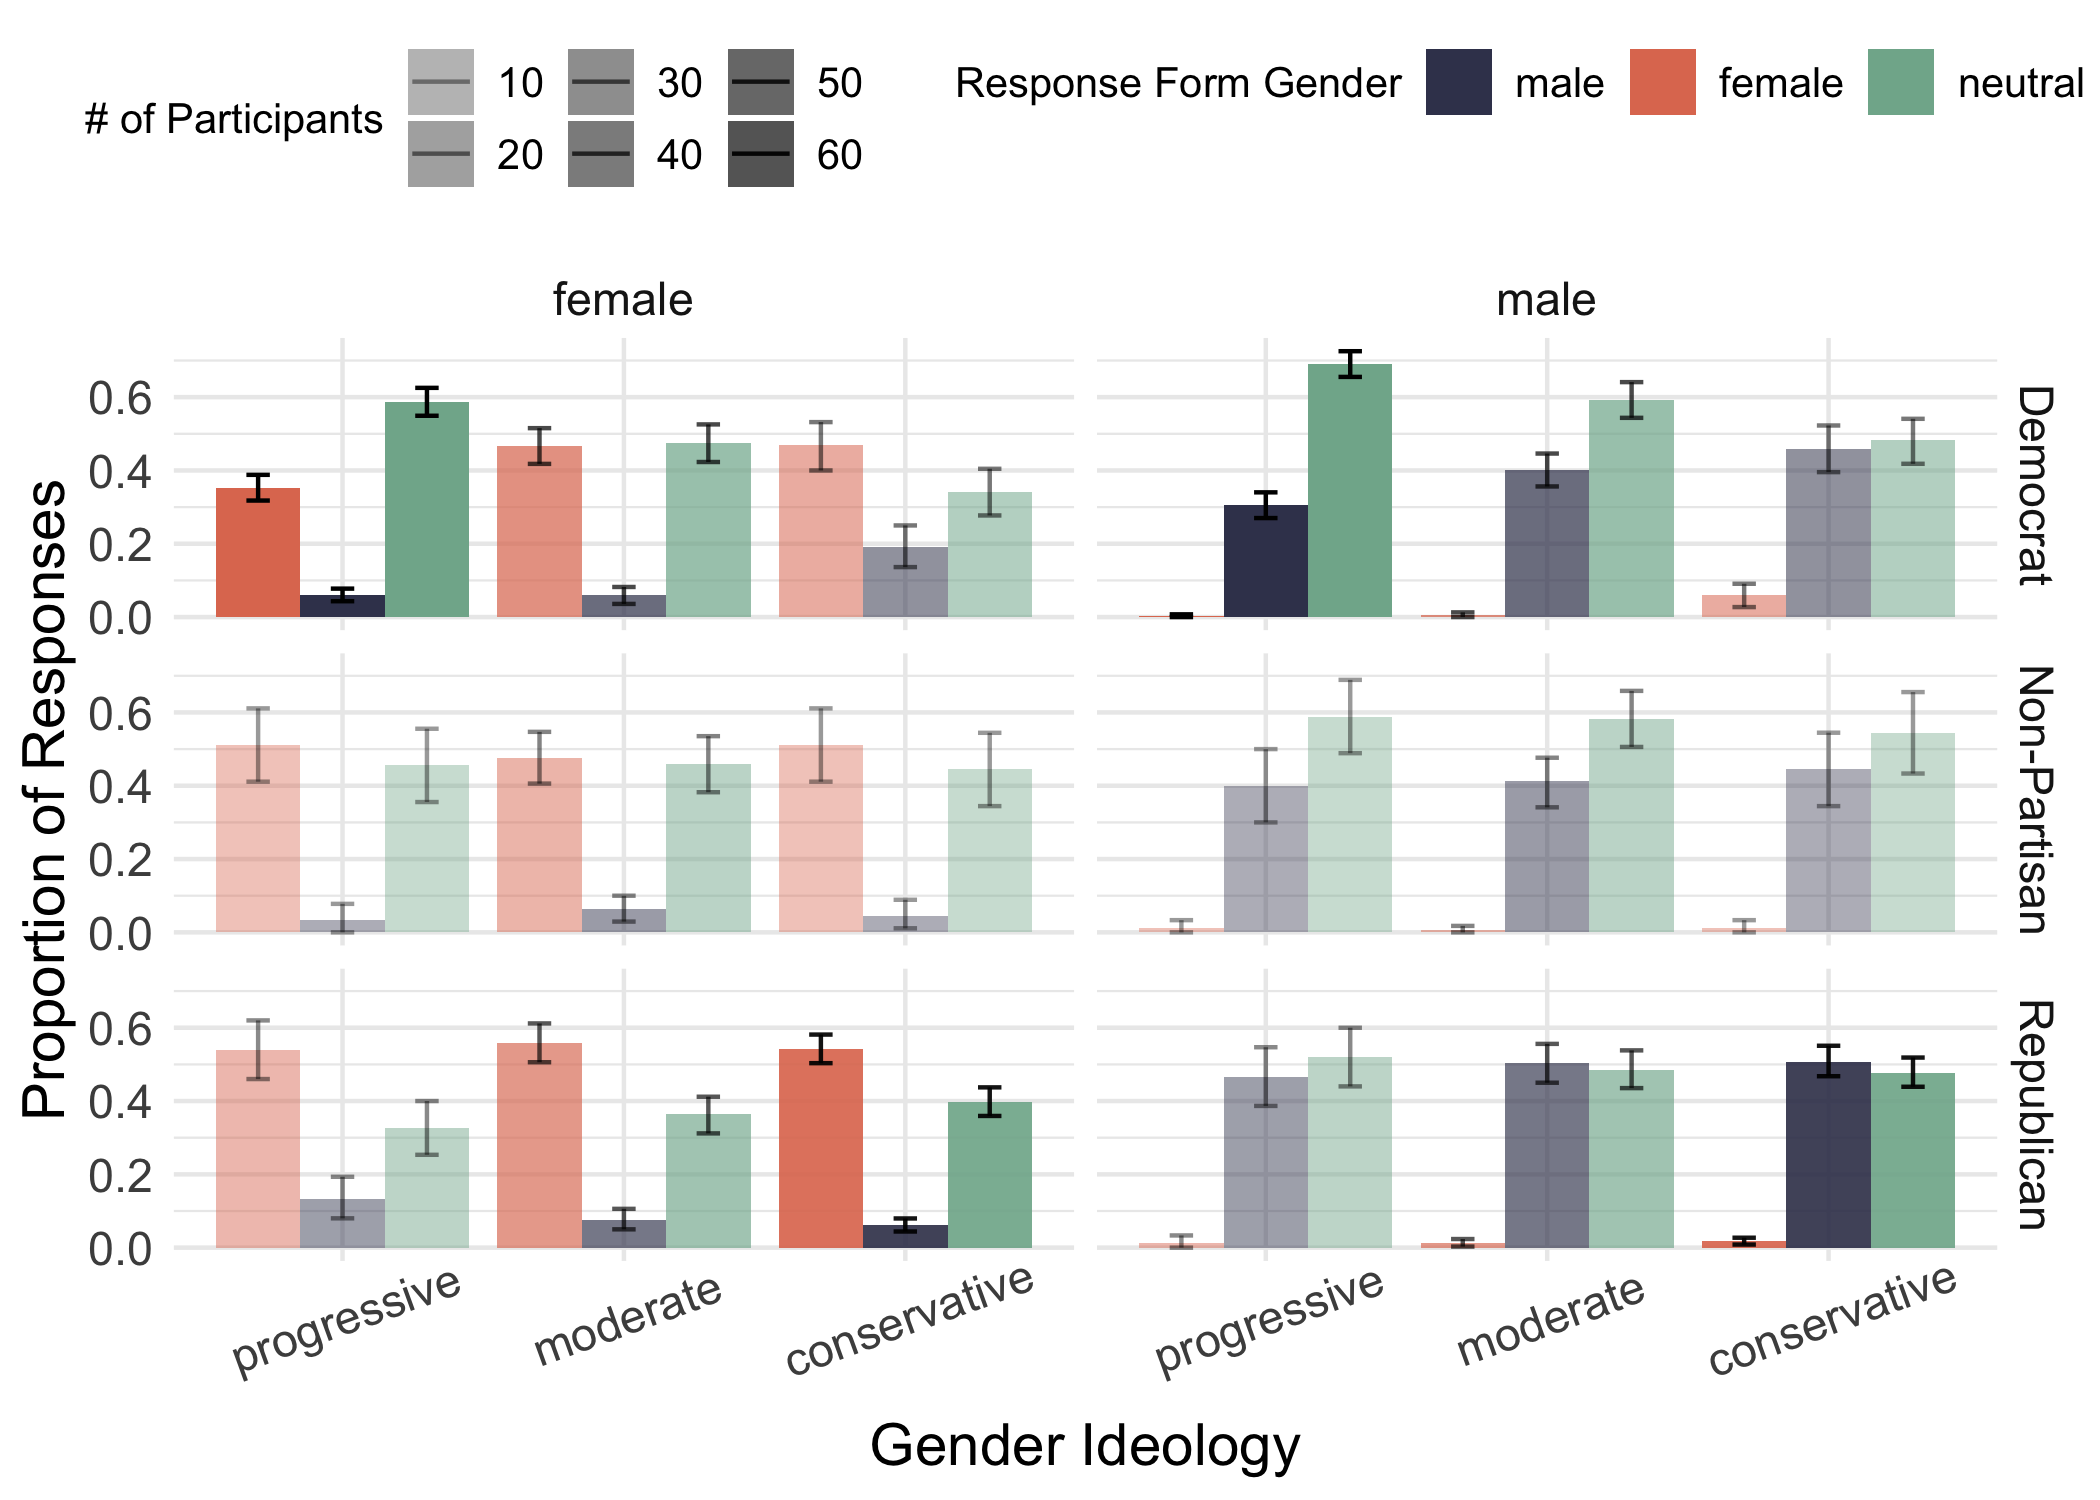
\includegraphics[scale=0.12]{prod-3x2x3.png}
		\caption{Proportion of responses by gender produced in Experiment Two, according to gender of the name in the stimulus sentence (x-axis facet) and participant political alignment (y-axis facet)}
	\end{figure}
		
	\begin{table*}[t!]
		\centering
		\caption{Model outputs for each fixed effect (rows) for each of the political macrocategories.}
		\vskip 0.12in
		\begin{tabular}{l r r l r r l r r l }
			%		\begin{tabular}{l {p{2cm} r  p{2cm} r p{2cm} l p{2cm} r p{2cm} r p{2cm} l p{2cm} r p{2cm} r p{2cm} l }
					\toprule
					& \multicolumn{3}{c}{Democrats} & \multicolumn{3}{c}{Non-Partisans} & \multicolumn{3}{c}{Republicans} \\ \cmidrule(r){2-4} \cmidrule(r){5-7} \cmidrule(r){8-10}
					& \multicolumn{1}{c}{$\beta$} & \multicolumn{1}{c}{SE} & \multicolumn{1}{c}{p} & \multicolumn{1}{c}{$\beta$} & \multicolumn{1}{c}{SE} & \multicolumn{1}{c}{p} & \multicolumn{1}{c}{$\beta$} & \multicolumn{1}{c}{SE} & \multicolumn{1}{c}{p}\\ 
					\midrule
					trial gender   & 0.862 & 0.124 & \cellcolor{lightgray} $<$0.001        & 1.041 & 0.223 & \cellcolor{lightgray} $<$0.001 & 1.272  & 0.143 &  \cellcolor{lightgray} $<$0.001\\
					ideology & -0.034  & 0.007 & \cellcolor{lightgray} $<$0.001            & -0.005 & 0.015& 0.714           & 0.001  & .005 & 0.886 \\
					log odds & 9.234 & 2.222  &  \cellcolor{lightgray} $<$0.001            & 15.242 & 4.623 & \cellcolor{lightgray} $<$0.001     & 14.596  & 2.315 & \cellcolor{lightgray} $<$0.001\\
					\bottomrule
				\end{tabular}
				%\caption{lmer(suspectconvictionJustified ~ generation * condition + (1|storyreproduction), data=dfmodel); high correlation of fixed effects}
				\label{tab:exp2results}
			\end{table*}
		
	\subsubsection{Referent Gender} With regard to trial gender, or the gender of the name presented in the vignette, we observed a main effect on production rates of gender-neutral titles. This resulted in participants of all three political macrocategories being more likely to produce gender-neutral forms when forced to pick a role title that coreferred with a male name. Across all observations, gender-neutral forms were produced 57\% of the time with male names, compared to only 48.7\% of the time with female names. These trends are presented in Row 1 of Table 3, and shown in the cross-gender differences of Figure 3.
	

	
	\subsubsection{Log Odds} Finally, we observe a main effect of log odds in the expected direction, such that a higher log probability of the neutral occurrence predicts a neutral response selection. This effect was found across all three political macrocategories, as seen in the third row of Table 3.

	
	\section{General Discussion}
	 In our processing study, we observed no significant effect of gender ideology on the processing of gender-neutral role titles when they coreferred with gendered names. This is reminiscent of the findings of \textcite{von2020implicit}, wherein presidentially-coreferential \textit{she} incurred a significant processing penalty despite societal expectations that Hillary Clinton would win the 2016 election. Our data similarly indicates individually-held beliefs about gender do not modulate the processing of gender-neutral role nouns.\par 
	This finding is particularly intriguing when contrasted with the findings of our production task. When forced to make a gendered selection of a role noun which corefers with a gendered name, we observe that gender-progressive Democrats are more likely to select the gender neutral version than their more conservative counterparts. This is true both group internally (i.e. progressive Democrats use neutral terms more than conservative Democrats) and group-externally (i.e. Democrats use more neutral terms than Republicans or Non-Partisans). Taken together with the results of \textcite{pozniak2021failures}, it appears that individual expectations about events or gender roles do indeed modulate the production of gendered language.\par 
	To explain this two-part discrepancy, we appeal to the notion of \textit{indexicality} \parencite{eckert2008variation}. We argue that gender-neutral forms of morphologically-gendered items are a semiotic resource upon which users of English can draw to index their relative progressiveness with regard to gender. As a result, Democrats (who have generally higher scores on our scale of gender-progressiveness) are more likely to use gender-neutral compounds in their creation of gender-progressive personae. On the other hand, Republicans are less likely to use these forms, as doing so would index an ideology about gender that they may not have. This seems at least numerically substantiated in our data, as the Republicans also had a more conservative score on the gender ideology index. \par 
	The existence of overt commentary on the employment of gender-neutral role titles in the public sphere further substantiates this interpretation. For example, Richard Grenell, former Acting Director of National Intelligence under President Trump, tweeted an image of a gingerbread person with an accompanying display-case card that read ``Gingerbread Person". Alongside this was Grenell's caption `Stop voting for Democrats.' \parencite{Grenell}. Here, Grenell explicitly draws on the Democrat association with gender neutral role nouns in order to implicitly assert that elected Democrats are responsible for the proliferation of politically-correct language regarding gender. In this sense, then, we argue that the production of gender-neutral forms has come to index a stance of gender progressiveness, and that such indexical associations form part of a larger language ideology (in the sense of Gal \& Irvine 1995) wherein differences in gendered language are mapped onto social categories such as `Democrats' or `Republicans'.\par 
	We also observe that male names are more likely to elicit neutral role titles in the production task than female names. We posit that this may be because the lexical items under investigation are overwhelmingly male-associated, with only \textit{flight attendant} being rated as `likely a woman' in the results of our norming study (see Supplementary Materials). As a result, these roles being filled by women are societally `marked', in that they run counter to our expectations. Participants may then be more likely to pick the `marked' form of the lexeme, which in most cases is the female form, either by morphology (\textit{actor} vs. \textit{actr-ess}, where \textit{actress} is morphologically more complex) or by frequency. While none of the participants in our norming study reported being unfamiliar with any of the female terms (see Supplementary Materials), terms such as \textit{firewoman} and \textit{villainess} are rare in the corpus, if they occur at all (\textit{firewoman}, for example, does not). As such, it may be the case that participants are selecting marked linguistic forms to pick out marked real-world referents.\par 
	Alternatively, as is apparent in Figure 4, the answer may partially lie in the fact that respondents are willing to assign female referents masculine titles at a much greater rate than they are to do the opposite. While such productions were not included in the analysis, their presence as options in the task at hand may have inadvertently skewed the proportions of productions. Future work is planned to investigate these `gender incongruent' productions.\par 
%	Finally, we observe in the processing task that the effect of frequency is markedly more predictive for the young participants than it is for the older participants. While not directly related to the question at hand, it bears mentioning here due to the politically charged nature of the data. One possible interpretation of this finding is that young people are not consuming the kinds of mainstream media that are reflected in COCA, and as such are not receiving the same kind of input on politically charged terms as their elders. If this is the case, it has larger-reaching implications for the ways in which we implement frequency estimations into our linguistic analyses, and we believe this discrepancy and the related line of inquiry deserve further investigation. \par 
	In sum, we believe that these results further our understanding of the relationship between gender and language by highlighting an incongruity in the processing and production of gender-neutral role nouns. Moreover, this incongruity is found at the individual level, calling for a greater degree of granularity of our investigations of biases in the linguistic system. The examination of such biases is critical in the development of fair and inclusive language, and we hope that the work herein will encourage researchers to pursue such work with the individual and their experiences in mind. 
	

	\newpage
	\nocite{gal1995boundaries}
	\printbibliography
	
	
	
\end{document}